\documentclass[11pt]{article}
% Shared preamble for the course handouts and the cheatsheet (article class).
\usepackage[T1]{fontenc}
\usepackage[utf8]{inputenc}
\usepackage{lmodern}
\usepackage[a4paper, margin=2cm]{geometry}
\usepackage{amsmath, amssymb, bm, booktabs, graphicx, xcolor, enumitem, tcolorbox, multicol, listings}
\usepackage{tikz}
\usetikzlibrary{arrows.meta, positioning, calc}
\usepackage[hidelinks]{hyperref}
\setlength{\parindent}{0pt}
\setlength{\parskip}{0.5em}

% same colours and macros as the slides (slides/preamble.tex)
\definecolor{accent}{HTML}{C0392B}
\definecolor{cool}{HTML}{2E6DB4}
\definecolor{muted}{HTML}{7A7A7A}
\definecolor{good}{HTML}{2E8B57}
\definecolor{prob}{HTML}{E67E22}
\newcommand{\given}{\,|\,}
\newcommand{\E}{\mathbb{E}}
\newcommand{\KL}[2]{D_{\mathrm{KL}}\!\left[#1\,\middle\|\,#2\right]}
\newcommand{\N}{\mathcal{N}}
\newcommand{\Hess}{\mathcal{H}}
\DeclareMathOperator*{\argmin}{arg\,min}

% boxes
\newtcolorbox{keyidea}{colback=accent!5, colframe=accent!70!black, boxrule=0.6pt, arc=2pt, left=6pt, right=6pt, top=4pt, bottom=4pt}
\newtcolorbox{labhelp}[1]{colback=good!5, colframe=good!60!black, boxrule=0.6pt, arc=2pt, title={\small\bfseries #1}, fonttitle=\small, left=6pt, right=6pt, top=4pt, bottom=4pt}
\newtcolorbox{backupbox}[1]{colback=cool!5, colframe=cool!70!black, boxrule=0.6pt, arc=2pt, title={\small\bfseries #1}, left=6pt, right=6pt, top=4pt, bottom=4pt}

\lstset{basicstyle=\ttfamily\small, columns=fullflexible, keepspaces=true, showstringspaces=false,
  commentstyle=\color{muted}, keywordstyle=\color{cool}\bfseries, language=Python, frame=none,
  backgroundcolor=\color{black!3}, xleftmargin=4pt, aboveskip=4pt, belowskip=4pt}

\graphicspath{{../slides/figures/}}
\setlength{\parskip}{0.28em}\linespread{0.94}
\setlist{nosep}
\emergencystretch=2em
\tcbuselibrary{breakable}
\tcbset{breakable,left=5pt,right=5pt,top=3pt,bottom=3pt}
\usepackage{longtable,array}
\newcommand{\nat}{\,\text{nats}}
\newcommand{\slt}[1]{\emph{#1}}   % slide title
\newcommand{\norm}[2]{\lVert #1\rVert^2_{#2}}
\newcommand{\dens}{\varrho}

\title{\textbf{A robot that acts to know}\\[0.3em]\large Day 4 handout --- One concept, from birth to action: the chair}
\author{}
\date{Thursday 3 December}

\begin{document}
\maketitle
\vspace{-2em}

\noindent
On Day 3 the robot's belief became a set of pieces on a shared graph, each piece owned by one agent. Today we follow two of those pieces through their whole life, and in both we do only one thing, lower the free energy $F$ of Day 2. The first piece is the robot's own pose in a room whose walls are given (Example 1). The second is a chair: how a chair is born in the belief, how its position is sharpened, how it is removed when it is gone, and how it is forgotten (Example 2). Both examples have the same shape: a prior (what the robot believed before), a likelihood (what the sensors say now), and a solver that finds the belief that lowers $F$. Both examples are shown in simulation only. In the last part we ask what the robot should do next, and the answer is again a number in nats: the expected free energy $G$ of each look it could take.

Section~1 follows the slides in order and writes out every step the slides only show. The backup slides are in blue boxes where they belong. Section~2 is a guide to each of the 22 lab exercises. Section~3 is a glossary. Slide titles are in italics. The numpy and probability tools are in the cheat sheet (\texttt{cheatsheet.pdf}) and are not repeated here.

\paragraph{Notation used in this handout.} $s$: the distance to a wall; $o$: a reading; $\mu$: the belief about $s$; $a$: the robot's speed. $X=(x,y,\varphi)$: the robot's pose in the room frame; $\bar X,\bar P$: the pose and covariance predicted from the wheels; $P$: the covariance after the update. $d(p)$: the distance from a point $p$ to the nearest wall. $q_n$: LiDAR return $n$ in the robot's frame; $p_n(X)$: the same return placed in the room by pose $X$; $d_n(X)=d(p_n(X))$; $\sigma$: the noise of one such distance; $w_n$: how much the model explains return $n$, a number between 0 and 1. $\theta=(x,y,\psi)$: a chair's pose. $\rho(u)=-\ln p(u)$: the cost of a residual of $u$ standard deviations (Huber in the localiser, ``chair or clutter'' for the chair). $\|v\|^2_M=v^\top M v$. $L$: the existence log-odds of an object. $\Delta H$: entropy removed by a look, in nats. $G$: expected free energy. A \emph{nat} is the unit of $-\ln p$: a difference of $k$ nats is odds of $e^{k}$ to 1.

%=====================================================================================
\section{The lecture}
%=====================================================================================

\subsection{Perception and action both lower $F$; the goal goes in the prior}

\paragraph{One $F$, two handles.} \slt{Perception moves the belief, action moves the robot: both lower $F$.} A robot is 1.0 m from a wall by its belief ($\mu=1.0$) but reads $o=1.5$ m. We write the model: the sensor noise is $0.2$ m, so the likelihood is $\N(o;s,0.2^2)$ with precision $1/0.2^2=25$; and the \emph{goal} is written as a prior, $p(s)=\N(1.0,\,0.5^2)$ (``I expect to be 1 m from the wall, give or take 0.5 m''), precision $1/0.5^2=4$. Up to constants, $F=-\ln(\text{prior}\times\text{likelihood})$ is
\[
F=\tfrac12\cdot 25\,(o-\mu)^2+\tfrac12\cdot 4\,(\mu-1)^2 .
\]
At the start $F=\tfrac12\cdot25\cdot0.5^2=3.125$. There are two ways to lower it.
\begin{itemize}
\item \textbf{Perception} changes $\mu$ and leaves $o$ alone. Setting $\partial F/\partial\mu=25(\mu-o)+4(\mu-1)=0$ gives $\mu=(25\cdot1.5+4\cdot1)/29=1.431$, the precision-weighted average of Day 2. Then $F=\tfrac12\cdot25\cdot0.069^2+\tfrac12\cdot4\cdot0.431^2=0.431$. The robot can go no lower by thinking.
\item \textbf{Action} changes $o$ and leaves the model alone. The robot drives 0.5 m towards the wall; now $o=1.0=\mu$ and $F=0$.
\end{itemize}
The number 0.431 is the \emph{surprise} $-\ln p(o)$ (up to a constant): the reading $o$ has distribution $\N(1,\,0.2^2+0.5^2)$ under the model, so $-\ln p(o)=\tfrac12\,0.5^2/0.29=0.431$. Day 2's identity $F=\KL{q}{p(s\given o)}-\ln p(o)$ now reads: the belief term (how wrong $q$ is) is $3.125-0.431=2.694$ nats, and perception removes it; the surprise term can only be changed by changing $o$, that is, by acting. (The slide prints 2.67 because it subtracts the rounded values 3.1 and 0.43.)

\paragraph{The loop, every 0.1 s.} \slt{Put the goal in the prior: the robot drives until it comes true.} The robot (1) reads $o$; (2) moves $\mu$ downhill on $F$, $\dot\mu=-\partial F/\partial\mu$; (3) changes the speed $a$ downhill on $F$. The speed acts on $F$ only through the next reading: driving at $a$ for 0.1 s changes $o$ by $0.1\,a$, so $\partial o/\partial a=0.1$ s and
\[
\dot a=-\frac{\partial F}{\partial o}\,\frac{\partial o}{\partial a}=-25\,(o-\mu)\cdot 0.1 .
\]
A reading above the belief gives a negative speed, which on the slide's plot means towards the wall. Starting 2.6 m away, the prior keeps $\mu$ a little nearer 1 m than $o$, the robot drives in, and both end at the goal. There is no separate ``go to 1 m'' command: the goal is part of the model, and acting makes the model true.

\begin{keyidea}
Perception lowers $F$ by changing the belief, down to the surprise. Only action lowers the surprise, by changing the reading. A goal is a prior: the robot is surprised away from it, and drives until it is not.
\end{keyidea}

%=====================================================================================
\subsection{Example 1: the robot in its room}
%=====================================================================================

\paragraph{The setting.} \slt{The robot starts in three rooms it has never seen.} At the start the robot knows no walls, no furniture and no doors; its drive is to build a model of the place, one room at a time, and ``as close as it can'' is measured by $F$. Building the room itself (the walls, found with no map) is in the backup boxes and in optional lab Exercises 7--11. For the main line, the room is given as a polygon, and the question is where the robot is inside it.

\paragraph{The distance field.} \slt{The room supplies the likelihood: each laser return has a distance to a wall.} Once per room we compute, at every point $p$ of a grid, $d(p)=\min_k \mathrm{dist}(p,\text{wall}_k)$, the distance to the nearest wall. It is zero on a wall and grows linearly away from it; its slope $\nabla d$ is a unit vector pointing away from the nearest wall, so it says which way a point must move to get closer. The code calls $d$ an SDF (signed distance field), but on a room outline it is \emph{unsigned}: it has no inside or outside, so it cannot tell a robot that has drifted out of the room from one inside it.

Each scan gives returns $q_n$ in the robot's frame. If the pose is $X=(x,y,\varphi)$, return $n$ lands in the room at $p_n(X)=R(\varphi)\,q_n+(x,y)$, where $R(\varphi)$ is the rotation by $\varphi$. A return that hit a wall should sit on that wall, so $d_n(X)=d(p_n(X))$ should be 0: it is the \emph{prediction error}. No expected scan is drawn; the room turns a pose directly into a list of errors.

\paragraph{Localising is lowering $F$ over the pose.} \slt{Localising is lowering $F$ over the pose.} We write the model as a prior on the pose, $\N(\bar X,\bar P)$, and a likelihood in which each distance is zero up to noise, $d_n\sim\N(0,\sigma^2)$. Then $F(X)=-\ln(\text{prior}\times\text{likelihood})$ up to constants is
\[
F(X)=\underbrace{\tfrac12\,(X-\bar X)^\top\bar P^{-1}(X-\bar X)}_{\text{prior: where the wheels say}}+\underbrace{\frac1{2\sigma^2}\sum_n d_n(X)^2}_{\text{likelihood: every return onto its wall}} .
\]
\emph{We write} this model; \emph{the robot computes} the pose $X$ that lowers $F$ (the solver finds the minimum), and how sure it is. The slope of $d_n$ with respect to the pose is $g_n=\partial d_n/\partial X=\nabla d(p_n)^\top\,[\,I_2\ \ \mathrm{perp}(p_n-t)\,]$, with $t=(x,y)$ and $\mathrm{perp}(v)=(-v_y,v_x)$: moving the robot by $\delta$ moves the return by $\delta$, and turning it by $\delta\varphi$ moves the return sideways by $\delta\varphi$ times its distance from the robot.

\paragraph{Why the curvature is the covariance.} Near the minimum $X^\ast$ the slope of $F$ is zero, so $F(X)\approx F(X^\ast)+\tfrac12(X-X^\ast)^\top H\,(X-X^\ast)$, where $H$ is the matrix of second derivatives (the curvature). The belief is $q\propto e^{-F}$, which is a Gaussian with covariance $H^{-1}$. This is Day 2's Laplace rule, and the robot reports $P=H^{-1}$. For our $F$ the curvature, built from the first derivatives $g_n$ only, is
\[
H=\bar P^{-1}+\frac1{\sigma^2}\sum_n w_n\,g_ng_n^\top .
\]
Each return adds a precision $1/\sigma^2$ along $g_n$, the normal of its wall, and nothing along the wall. A single wall therefore says nothing about where the robot is \emph{along} it; the pose is pinned only because the room has walls with different normals, and because corners (below) add more.

\begin{center}
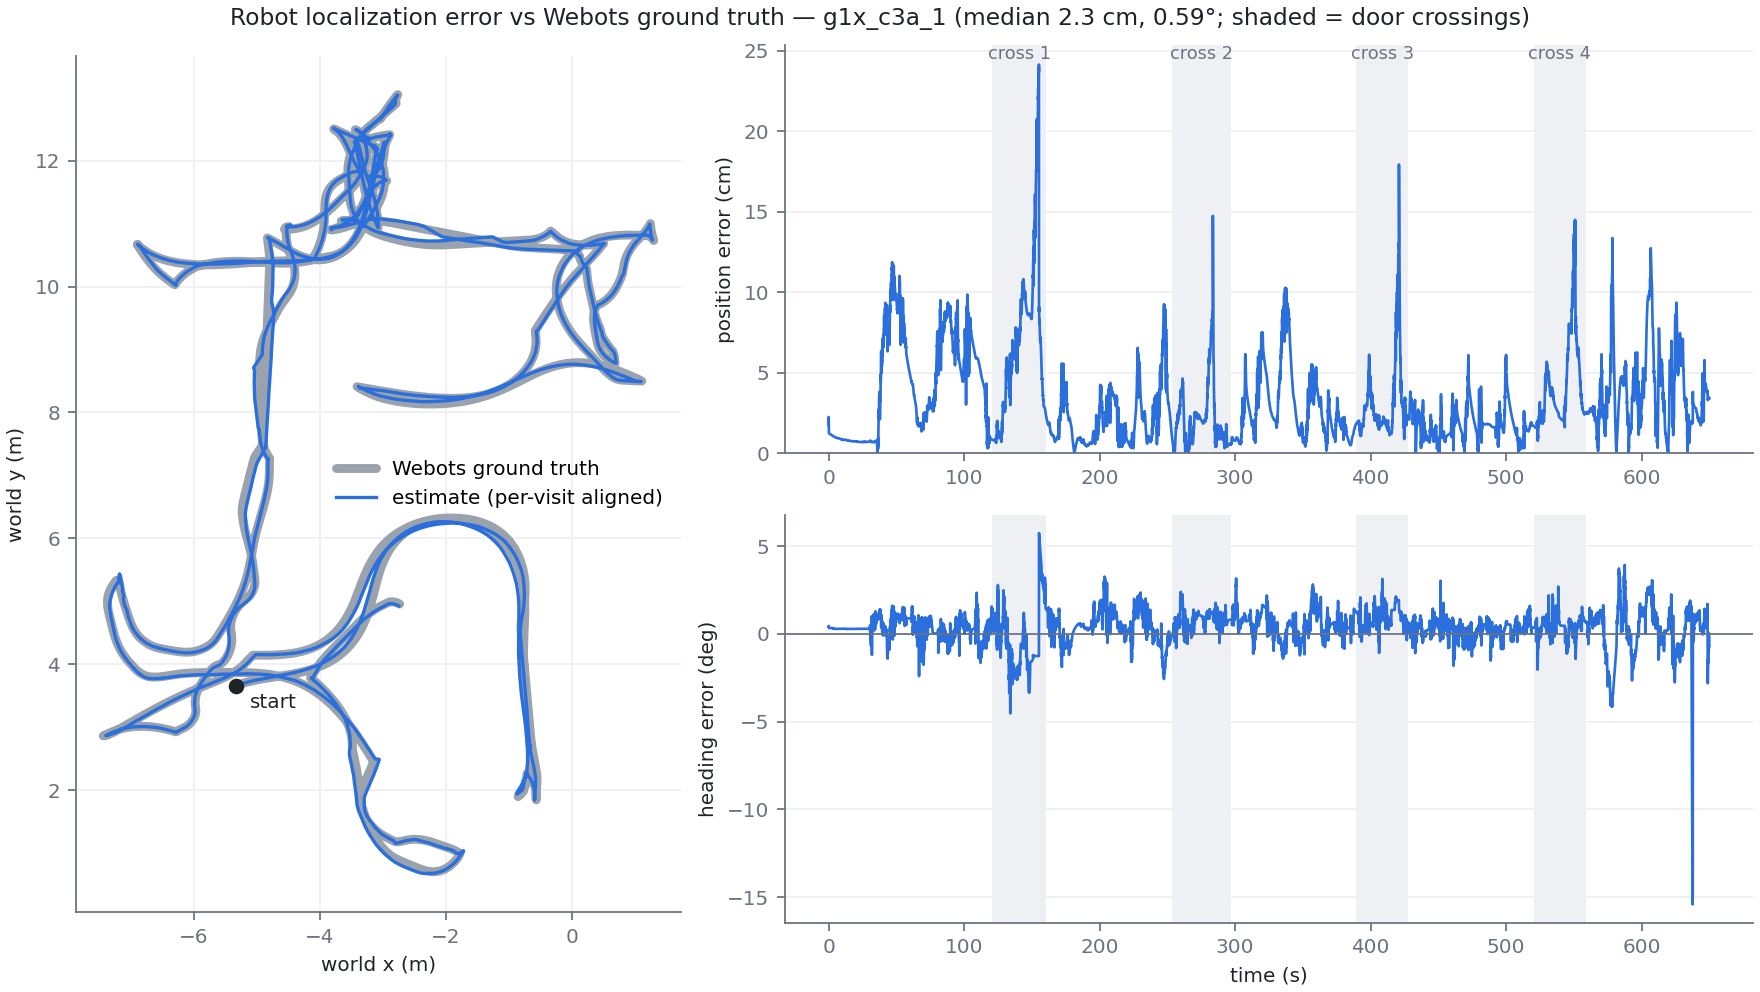
\includegraphics[height=3.4cm]{d4_loc_error_sim.png}
\end{center}
\vspace{-0.6em}
\emph{Measured, simulated Webots tour (650 s, four door crossings):} the pose stays within centimetres of the truth, median error 2.3 cm and 0.6$^\circ$, with peaks at the door crossings. The real robot has no ground truth, so there is no such curve for it. (The toy lab is one room without doors and gives millimetres; not comparable.)

\subsubsection*{One cycle of the localiser}

\paragraph{Step 1: predict from the wheels.} \slt{Inside $F(X)$: one cycle of the localiser, step by step.} The wheels give $u_t$ (a distance and a turn). The predicted pose is $\bar X=f(X_{t-1},u_t)$. Its covariance comes from linearising $f$: if $X_{t-1}$ is off by $e$ and $u_t$ by $\varepsilon$, then $f$ is off by about $J e+J_u\varepsilon$, where $J=\partial f/\partial X$ and $J_u=\partial f/\partial u$ are the Jacobians (how the prediction moves with each input). A linear map $A$ of an error with covariance $\Sigma$ has covariance $A\Sigma A^\top$, and the two errors are independent, so
\[
\bar P = J\,P_{t-1}\,J^\top + J_u\,Q\,J_u^\top ,
\]
with $Q$ the covariance of the wheels' noise. For a robot that moves a distance $\Delta s$ and turns $\Delta\varphi$, with $\psi=\varphi+\Delta\varphi/2$, $f=(x+\Delta s\cos\psi,\;y+\Delta s\sin\psi,\;\varphi+\Delta\varphi)$ and
$J=\bigl(\begin{smallmatrix}1&0&-\Delta s\sin\psi\\0&1&\Delta s\cos\psi\\0&0&1\end{smallmatrix}\bigr)$. The doubt grows only because the wheels cannot say better; no constant noise is added at each step.

\paragraph{Steps 2 and 3: place each return, measure its distance.} Compute $p_n(X)=R(\varphi)q_n+(x,y)$ and then $d_n=d(p_n)$, by looking up the field. Lab Exercise 12 writes these two steps.

\paragraph{Step 4: weigh each return.} A return may be on the room's wall, or on clutter: a chair, a person. The running localiser weighs each return with the Huber cost. We write the cost of a distance as $\rho_H(d)=d^2/2$ for $|d|\le\delta$ and $\delta(|d|-\delta/2)$ beyond, with $\delta=0.15$ m (\texttt{HuberDelta}). Its slope is $d$ inside $\delta$ and $\pm\delta$ outside. A weighted square $w\,d^2$ has slope $w\,d$, so the two agree when
\[
w_n=\min\!\big(1,\;\delta/|d_n|\big):
\]
full weight within 15 cm of a wall, and falling like $1/|d_n|$ beyond. A return on a chair 0.3 m from the wall has $w=0.5$; at 1 m, $w=0.15$. It is never zero: a far return keeps a bounded pull (its slope never exceeds $\delta$), and is weighed, not thrown away.

\textbf{The lab's version, and the chair agent's, is a mixture.} We write the wall and the clutter as two explanations of $d_n$. Clutter is spread uniformly over the room's area $A$, so its density is $1/A$. A wall puts its returns along its length $\ell$ with Gaussian spread $\sigma$ across it, so its density is $\frac1{\ell}\N(d_n;0,\sigma^2)$. Their ratio is
\[
\dens_n=\frac{p(\text{wall})}{p(\text{clutter})}=\frac{A}{\ell\sqrt{2\pi}\,\sigma}\,e^{-d_n^2/2\sigma^2},
\]
and, with equal prior chances, the probability that the return came from the wall is $w_n=\dens_n/(1+\dens_n)$ (the lab's code calls the ratio \texttt{rho}). It is close to 1 on a wall and close to 0 far from every wall. With the lab's numbers $A=24$ m$^2$, $\ell=20$ m, $\sigma=2$ cm we get $A/(\ell\sqrt{2\pi}\sigma)=23.9$, and $w_n$ is 0.96 on the wall, 0.76 at 4 cm, \textbf{0.5 at 5.0 cm}, 0.21 at 6 cm and $9\times10^{-5}$ at 10 cm. The place where this weight falls ($\dens_n=1$) is set by the area and wall length through the model, not by a tuned number. Lab Exercise 12 uses the mixture.

\textbf{Question on the slide:} a chair stands between the robot and a wall; what do its returns do to the pose? \textbf{Answer:} little. They are far from every wall, so Huber gives them $w=\delta/|d_n|$, a small weight and a bounded pull: they are weighed, never thrown away. (With the lab's mixture the weight is about 0.)

\paragraph{Step 5: lower $F$.} Put the weights in $F(X)=\tfrac12\|X-\bar X\|^2_{\bar P^{-1}}+\frac1{2\sigma^2}\sum_n w_nd_n(X)^2$ and let the solver find the bottom $X_t$; then the curvature gives $P_t=H^{-1}$. The weights depend on the pose, so they are recomputed and the fit repeated (the lab does it three times).

\subsubsection*{The full loss over a window of poses}

\paragraph{The loss in words.} \slt{The full loss: walls now, corners from the last poses, wheels between them.} The running localiser does not estimate one pose but a window of five, $X_0,\dots,X_4$ ($X_4$ is the newest), each at least 10 cm or $9^\circ$ from the last. The loss is a sum of four terms: \textbf{walls} (the newest scan only, at $X_4$) $+$ \textbf{corners} (all five poses) $+$ \textbf{wheels} (between consecutive poses) $+$ \textbf{prior} (what the dropped poses left). The formula and the meaning of each symbol are in the backup box \slt{The full loss, written out} below.

\paragraph{Old corners and the chain.} The corner term of pose $k$ involves only $X_k$ (the corners $C_j$ are constants), so it can reach $X_4$ only through the wheel factors between them. In one dimension: a corner at pose $X_3$ fixes it to variance $\sigma_c^2$; one wheel step to $X_4$ adds $\sigma_w^2$; so that corner says of $X_4$ only $\sigma_c^2+\sigma_w^2$, and a corner $m$ steps back says $\sigma_c^2+m\,\sigma_w^2$: the farther back, the less it helps. In SLAM the same corner would be an unknown landmark, and seeing it from $X_1$ and $X_4$ would tie the two poses together directly (a \emph{loop}). Here the corner is fixed, so each sighting ties one pose to the room and to nothing else: the cycles pose--corner--pose are not SLAM loops.

\textbf{Question on the slide:} why keep corners from past poses but walls from the newest scan only? \textbf{Answer:} a corner is a few numbers per pose and is cheap to keep; a scan is thousands of points. (A scan still counts once more, when its pose leaves, through the prior.) The old corners still correct $X_4$ along the chain of wheel factors.

\begin{center}
\fbox{\parbox{0.92\linewidth}{\small\textbf{Video 1: the window of poses growing (40 s, no sound).} An L-shaped room with fixed corners; the robot drives a loop. Each time it has moved enough, a new pose joins the window, linked to the previous pose by a wheel factor and to each room corner it sees by corner factors. Only the newest pose carries a wall term (its scan, drawn as hits on the walls). With five poses in the window, the next pose pushes the oldest out: it fades, and what it knew becomes the prior on the new oldest pose.}}
\end{center}

\begin{backupbox}{Backup: \emph{The full loss, written out}}
We write it without the factor $\tfrac12$ of each squared norm, as the slide does:
\begin{align*}
F={}&\underbrace{\sum_n\rho\big(d_n(X_4)\big)}_{\text{walls: newest scan only}}
+\underbrace{\sum_{k,j}\rho\big(\lVert\hat z_{kj}-c_j(X_k)\rVert_{\Lambda_{kj}}\big)}_{\text{corners, all 5 poses}}\\
&+\underbrace{\sum_{k=1}^{4}\norm{X_k-f(X_{k-1},u_k)}{Q^{-1}}}_{\text{wheels, between consecutive poses}}
+\underbrace{\norm{X_0-\mu_b}{\Lambda_b}}_{\text{prior from dropped poses}} .
\end{align*}
$d_n(X_4)$: distance from return $n$ of the newest scan, placed at $X_4$, to the nearest wall. $\rho$: the Huber cost, quadratic near zero and linear beyond $\delta=0.15$ m, so a chair or a person costs a bounded amount. $\hat z_{kj}$: corner $j$ measured from $X_k$ (two wall lines are fitted near it and intersected), in the robot's frame. $c_j(X_k)=R(\varphi_k)^\top(C_j-t_k)$: where the given room corner $C_j$ should appear from $X_k$. $\Lambda_{kj}$: the precision of the corner measurement, high across each wall and low along it; a corner is what separates two poses that fit the walls equally well. (A later backup writes $z$ for the seen and $\hat z$ for the predicted corner; here $\hat z$ is the seen one, as on the main slide.) $f(X_{k-1},u_k)$ and $Q$: the pose the wheels predict and its noise (step 1). $\mu_b,\Lambda_b$: the prior left by the dropped poses. When a pose leaves, the oldest pose is marginalised (Day 1's ``sum it out''), which leaves a Gaussian on the new oldest pose. In one dimension, if the dropped pose was fixed by its scan to variance $\sigma_c^2$ and linked to the next by wheels of variance $\sigma_w^2$, the prior on the next pose has variance $\sigma_c^2+\sigma_w^2$. On the robot it comes from the dropped pose's scans and wheel links, marginalised; its corners are not folded in.
\end{backupbox}

\begin{backupbox}{Backup: \emph{The room as a probability model}, four slides}
The variables: $o$ the laser scans, $X$ the poses, $\delta$ what the wheels measured, $m$ the room's structure (how many corners, which turns), $\theta_m$ the corners' coordinates for that structure. The wheel reading is always there and nothing in the room explains it, so we \emph{condition} on it: take it as given and spend no factor on its probability. Day 1's chain rule is exact in any order, with $\delta$ behind the bar in every factor: $p(o,X,\theta_m,m\given\delta)=p(o\given X,\theta_m,m,\delta)\,p(X\given\theta_m,m,\delta)\,p(\theta_m\given m,\delta)\,p(m\given\delta)$. The model is what we \emph{cross out}: once the poses and room are known, the wheels add nothing about the scans; the path follows the wheels one step at a time, $\prod_\tau p(X_\tau\given X_{\tau-1},\delta_\tau)$; the wheels say nothing about the corners or the shape. What remains is $p(o\given X,\theta_m,m)\prod_\tau p(X_\tau\given X_{\tau-1},\delta_\tau)\,p(\theta_m\given m)\,p(m)$. Bayes turns the forward model round: $p(X,\theta_m,m\given o,\delta)\propto$ likelihood $\times$ prior; the hidden constant is the same for every room, and its $-\ln$ is the free energy that step 5 compares.
\end{backupbox}

\begin{backupbox}{Backup: \emph{Estimating a room} (five steps) and \emph{the price of a corner}}
While the room is unknown the robot builds it as it drives: (1) \emph{where am I?} A hidden scan-to-map registration against a grid of hits gives the pose, with no walls involved. (2) \emph{What is free?} Each 5 cm cell counts the beams that passed through it and those that stopped in it; more hits than passes means matter. (3) \emph{Outline}, redrawn every second with no memory: wall directions come from multiplying each normal's angle by 4 and averaging; the free region's border is straightened into horizontal and vertical edges. (4) \emph{Drive where most is unseen}, until what is left is smaller than the robot. (5) \emph{Which outline becomes the room?} Bayes on the structure: $-\ln p(o\given m)\approx$ misfit of the best-placed outline $+\;\kappa$ per corner. The price per corner is the complexity term of Day 2: a coordinate known to $\sigma=3$ cm inside a room $L=10$ m across is one slot out of $L/\sigma\approx333$, costing $\ln333=5.8$ nats (odds of 333 to 1). With right angles a corner shares one coordinate with each neighbour, so $V$ corners need $V$ numbers, and two more corners (rectangle to L, 4 to 6) cost $11.6$ nats: they are kept only if the misfit drops by more. The room is thus the first belief born, with the same equation (misfit plus complexity per vertex); up to 60 recent outlines are kept and scored on all the evidence, and in 7 of 10 apartment runs the winner was not the last one drawn. While the room is unknown its outline never corrects the pose: a wrong wall would pull the pose, and the pulled pose would confirm the wrong wall.
\end{backupbox}

\begin{backupbox}{Backup: \emph{Walls are not enough} and \emph{Symmetry}; \emph{Localising against the room you just built}}
A $6\times4$ m rectangle looks the same after a half-turn about its centre, so the same scan fits the true pose and its half-turn image with the same $F$ (to within a fraction of a nat; Exercise 14 gives $-786.82$ for both). There is no downhill path between two such poses, so they are separate hypotheses: the agent lists them, chooses by evidence that is not symmetric (a corner, the previous pose), then refines. This is one of the few places where a threshold is the right design: it is defensible exactly when the alternative cannot be written as a covariance. Second, the room is a constant here, so its error is shared by every scan: moving the east wall 1.5 cm takes the mean NEES from about 2 to 90 where 3 is correct (Exercise 13).
\end{backupbox}

%=====================================================================================
\subsection{Example 2: the life of a chair}
%=====================================================================================

\paragraph{What the camera and the retina give.} \slt{The chair the camera sees, and the belief the chair agent keeps of it.} In the simulated ZED frame the retina's detector (YOLO) labels a region ``chair 0.87'': that is the \emph{mask}, pixels with a class and a score. Its pixels, with their depth, become the 3-D points the chair agent fits. The blue box is the belief: the agent's fitted box (0.48$\times$0.52$\times$1.03 m, $\sigma$ 2 cm) projected into the image; it sits 4.5 cm from the true chair. The mask is evidence in pixels; the belief is a box in the room, with its doubt.

\paragraph{The chair's $F$ is the localiser's $F$ with the roles swapped.} \slt{The chair's $F$ is the localiser's $F$ with the roles swapped.} The robot's pose is known from Example 1; the chair's is not. Again $F=-\ln(\text{prior}\times\text{likelihood})$: a prior (where I believed the chair was) and a likelihood (every mask point onto the chair).
\begin{center}\small
\begin{tabular}{@{}p{2.3cm}p{5.6cm}p{6.2cm}@{}}
\toprule
& the robot in its room & a chair in the room\\\midrule
unknown & pose $X=(x,y,\varphi)$ & pose $\theta=(x,y,\psi)$; shape: the class template\\
data & LiDAR returns $q_n$ & the mask's 3-D points $p_k$, placed with the robot's pose\\
distance & $d(\cdot)$ to the nearest wall & $s_\theta(\cdot)$ to the chair's surface at $\theta$\\
prior & where the wheels say, $\bar X,\bar P$ & the last belief, widened by $Q$ each frame a mask arrives, $\bar\theta,\bar P_\theta$\\
off-model data & a chair in front of a wall & a point on the floor or the wall behind\\
\bottomrule
\end{tabular}
\end{center}
$F(X)=\tfrac12\|X-\bar X\|^2_{\bar P^{-1}}+\frac1{2\sigma^2}\sum_nw_nd(X\oplus q_n)^2$ and $F(\theta)=\tfrac12\|\theta-\bar\theta\|^2_{\bar P_\theta^{-1}}+\frac1{2\sigma^2}\sum_kw_ks_\theta(p_k)^2$, where $X\oplus q_n$ is return $n$ placed at $X$, $\theta=(x,y,\psi)$ is the chair's position and heading, $p_k$ are the mask's 3-D points placed in the room with the robot's pose, $s_\theta(p)$ is the distance from $p$ to the chair's surface at $\theta$, and $\sigma$ is the noise of the frame, shared by its points. $w$ bounds a stray point's pull: Huber for the room, ``chair or clutter'' for the chair. The chair's prior is widened by $Q$ each frame a mask arrives and frozen otherwise. The shape is not fitted: it is the class template, and only the pose is estimated. The robot computes the $\theta$ that lowers $F$, with $P=H^{-1}$ as before. \textbf{Question on the slide:} what does the chair agent read from the robot to place its points? \textbf{Answer:} the robot's pose \emph{with its covariance}, at the time the image was taken (Day 3): a pose error moves every point of the mask together.

\paragraph{Why the points do not average out.} \slt{(Backup: The common-mode ceiling.)} If $N$ points share one pose error $\delta\sim\N(0,\Sigma_\delta)$ and each has its own noise $\sigma$, the mean offset along the surface's normal has variance $\sigma^2/N+j^\top\Sigma_\delta\, j$, where $j$ is how the offset moves with the pose. The first term falls with $N$; the second does not: a denser mask eventually stops helping, and the limit is the robot's pose error, not the number of pixels. Exercise 15 measures it.

\subsubsection*{Birth}

\paragraph{Birth is a comparison of two worlds, in nats.} \slt{A chair is born when one more object explains more than it costs.} Take $n$ detections that no existing chair explains. World A: nothing new here; each detection is clutter, uniform over the room of area $A$, so its probability density is $1/A$ and it costs $\ln A$ nats. World B: one more object $\theta_{n+1}$; each detection scatters about it. The difference of free energies is
\[
\Delta F=F_B-F_A=\underbrace{\E_q[-\ln p(\bar Z\given\theta_{1:n+1})]-\E_q[-\ln p(\bar Z\given\theta_{1:n})]}_{\text{accuracy gained by explaining the points}}+\underbrace{\KL{q(\theta_{n+1})}{p(\theta_{n+1}\given\ell)}}_{\text{complexity paid for the new object}} ,
\]
with $\bar Z$ the unexplained points and $\ell$ the class (``chair''). The object is born exactly when $\Delta F<0$. The complexity is not a penalty added by hand: it is the same term every living instance already pays, the price of narrowing the class prior down to this chair's own belief. The lab (Exercise 1) writes the same thing with the prior probability $p_0=0.1$ that a new object is here included: $F_{\text{with}}=-\ln p_0+F_{\text{Laplace}}$ and $F_{\text{without}}=-\ln(1-p_0)+n\ln A$, so the object must first pay $\ln\frac{1-p_0}{p_0}=2.2$ nats for existing at all. (Footnote on the slide: the running agent counts instead; see the next paragraph.)

Why $\Delta F$ eventually becomes negative with good detections: each one saves $\ln A$ minus what its scatter costs. For the lab's room, $A=24$ m$^2$, a detection with scatter $\sigma=5$ cm costs on average $\ln(2\pi\sigma^2)+1=-3.15$ nats, so it saves about $3.18+3.15=6.3$ nats; the price of the object grows only like $\ln n$. The lab gives $\Delta F=+2.9,\,-2.6,\,-9.2,\ldots$ for 1, 2, 3 sharp views, falling about 6.5 per view. A distant view ($\sigma=30$ cm) saves only about $2.8$ nats each (four views in this run). A reflection scatters over a 1.2 m patch while the detector reports $\sigma=10$ cm: each costs about 9.2 nats against 3.2 for clutter, so $\Delta F$ rises (57.8 after ten) and the object is never born. Over 300 runs, two sharp views are accepted by $\Delta F<0$ 98\% of the time and by a streak of three never (a streak needs three); ten reflections are accepted by the streak 94\% and by $\Delta F$ never. \slt{(Backup: A streak cannot read evidence.)} A streak counts frames; $\Delta F$ reads how sharp each frame was and how well the frames agree.

\paragraph{What actually runs: a count that stands in for the nats.} The lecture explains birth as a comparison in nats. The running chair agent does not compute $\Delta F$. It uses a count: a chair is born when a weighted count of observations reaches \texttt{BirthFrames} $=8$ (\texttt{chair\_concept/etc/config.toml}). Each observation is worth at most 1: its weight is the detector's confidence times a range factor, which is 1 up to 2.5 m and $(2.5/\text{range})^2$ beyond it (the pixel area of the object falls like $1/\text{range}^2$). A repeated frame (the same image counted twice), a smeared frame (taken while the robot drives past) or a truncated mask is worth 0. For example, a confidence 0.87 at 2 m is worth 0.87, so at least 10 observations are needed; at 5 m it is worth $0.87\times0.25=0.22$, so about 37; at 7 m with confidence 0.9, $0.9\times0.128=0.115$, so about 70. The count is a threshold, and the backup \slt{What the robot actually computes: a threshold that should not be one} says so: it is a product of sensible factors (confidence, range, admissible, shape, in the room, surprise) counted in frames, while death is counted in evidence, so birth cannot be traded against anything else. The count stands in for the nats comparison until the plumbing for $\Delta F$ exists; the lab's Exercise 2 uses a still simpler streak (three detections within 0.6 m) to show what a count cannot do.

\begin{center}
\fbox{\parbox{0.92\linewidth}{\small\textbf{Video 2: a chair's birth (30 s, no sound, illustrative numbers).} A 3-D room; the robot drives towards a chair, and its field of view is drawn as a cone on the floor. The chair's surface points it sees pile up as red, unexplained points. A panel on the right weighs two bars in nats. The blue bar is the \emph{accuracy}: the surprise a chair removes from the points, $\sum_i[-\ln p(z_i\given\text{clutter}) + \ln p(z_i\given\text{chair})]$. Clutter spreads a point evenly; the chair puts it near its surface, with a depth spread $\sigma(r)$ that grows as $r^2$ and equals the clutter spread at the sensor's range limit $R$, so one point is worth about $2\ln(R/r)$ nats (scaled down because points of one view share their error). Nearer views count more, so the bar climbs faster as the robot approaches. The red bar is the \emph{complexity}: the KL of the fitted belief from the class prior, about $c_0 + \tfrac32\ln(1 + n\,\sigma_\text{prior}^2/\sigma^2)$ for three unknowns after $n$ points; it grows slowly as the fit sharpens. The dashed line marks where the red bar ends. When the blue bar passes it (about 15\,s in) the chair's model, a blue box at its fitted pose, is born, and as the robot keeps looking the box sharpens.}}
\end{center}

\subsubsection*{Absence: a miss is evidence only where the object would have been seen}

\paragraph{Existence is one running number.} \slt{A miss is evidence only where the object would have been seen.} Every belief carries a log-odds $L=\ln\frac{P(\text{exists})}{1-P(\text{exists})}$. By Bayes, posterior odds are prior odds times a likelihood ratio, so each frame adds $\ln$(likelihood ratio) to $L$. A frame says one of three things. (i) \emph{Occupancy}: a return inside the believed volume. It confirms: $L$ goes up. (ii) \emph{Predicted visible, and nothing there}. It removes: $L$ goes down. (iii) \emph{Occluded, out of view, or too far to tell}. It holds: nothing changes. The size of (ii) comes from the model. If the object is there and the sensor would detect it with probability $P(\text{detect})$, then ``nothing seen'' has probability $1-P(\text{detect})$ if the object exists and $1$ if it does not, so the frame adds $\ln\big(1-P(\text{detect})\big)\approx-P(\text{detect})$: a miss counts in proportion to how likely the sensor was to see the object. Evidence for and against simply adds, and $L$ is capped short of certainty so that an object can always recover.

\paragraph{Cap, then weight.} \slt{A poor view must not remove an object, however many beams it has.} In the lab $L$ is kept between $-4$ and $+4$, starts at 2.0 and an object is removed below $-3.5$; these are toy values (the chair agent: birth 1.0, removal $-3.0$). The slide's rule is $\Delta L=-P(\text{detect})\cdot\min(c\,n,\ell)$: $n$ is the number of beams that should have landed on the object in this frame, $c$ what one beam is worth, $\ell$ the most one frame can say. In the lab $P(\text{detect})=1-\prod_{\text{beams}}(1-p_b(r))$ with $p_b(r)=e^{-(r/3\,\text{m})^2}$. Beams that would land on the object are found by ray-casting from the robot through everything the robot believes, \emph{including the walls}; without the walls, a chair in the next room projects into view, finds no detection, and votes for its own removal. (The backup \slt{A factor whose argument list was wrong} reports this defect in three agents.) The points of one frame are not independent, so one frame may move $L$ by at most $0.4$. The order matters: \emph{saturate, then weight}, $-P(\text{detect})\cdot\min(c\,n_{\text{pred}},0.4)$. Weighting the count first, $-\min(P(\text{detect})\,c\,n_{\text{pred}},0.4)$, does nothing for a view with many beams: a large object 40 beams wide, each beam only 0.05\% likely to fire, is a 2\%-resolvable view. Saturate-then-weight drops $L$ by $0.0198\times0.4=0.0079$; weight-the-count drops it by $\min(0.79,0.4)=0.4$, the full ceiling. \slt{(Backup: Weight absence by how visible it was, after the bucket.)} In words: weight a miss after the cap, otherwise many beams fill the cap however poor the view.

\paragraph{One tour.} \slt{One tour: only absence weighted by visibility removes just the vase.} The rows on the slide are: \emph{evidence}, $\Delta L=-P(\text{detect})\min(c\,n,\ell)$ with walls blocking the line of sight; \emph{no walls}, the same but visibility ignores walls; \emph{weight the count}, the weight applied before the cap $\ell$; \emph{miss counter}, every miss counts the same. A robot tours a living room holding five beliefs: a table, a bottle, a plant behind the table, a chair that is really in the next room, and a vase that someone removed. Removal by rule: the evidence rule removes the vase (frame 68) and nothing else; with no walls it also removes the chair (frame 174); weighting the count removes the vase at frame 13 (right object, but five times too soon, since a far view counts as fully as a near one); a miss counter removes everything by frame 44. An object that can never be probed is never removed: a constant decay would remove it, which is removal without evidence on the agent's clock. Instead, uncertainty that cannot be resolved from here is routed to a verification pull: the expected information of a view of it rises and the robot goes to look.

\subsubsection*{Forgetting}

\paragraph{A fixed doubt per frame forgets at one rate.} \slt{A fixed amount of doubt per frame forgets at one rate.} In the version measured here, the tracker adds a constant process noise $Q$ to the variance every frame, seen or not: $\Sigma\leftarrow\Sigma+Q$. On the slide $\sigma_w$ is the table's position spread, $\Sigma_0=(3\text{ cm})^2$ its variance when last seen, $Q=(5\text{ mm})^2$ per frame and $n$ the number of frames without points. Two consequences, neither of which depends on how long the object has been known. Unobserved, the variance grows linearly, $\Sigma(n)=\Sigma_0+Qn$. A table known to 3 cm ($\Sigma_0=9\times10^{-4}$ m$^2$), with the deployed $Q=(0.005\text{ m})^2=2.5\times10^{-5}$ per frame at 10 Hz, doubles its variance (halves its precision) after $\Sigma_0/Q=36$ frames, 3.6 s. Measured: a real table, 1320 blind cycles, predicted error $\sqrt{\Sigma_0+Qn}=0.184$ m, logged 0.170 m. Observed, precision stops at a floor. One predict and one update of information $i=1/R$ (the information of one frame) give in steady state $\Sigma=(\Sigma+Q)/(1+i(\Sigma+Q))$, that is $i\Sigma^2+iQ\Sigma-Q=0$, so $\Sigma\approx\sqrt{Q/i}$ and $\sigma_{\text{steady}}\approx(Q/i)^{1/4}$. With $R=0.02^2$: $(2.5\times10^{-5}\times4\times10^{-4})^{1/4}=10.0$ mm (the full quadratic gives 9.4 mm, which is what the simulation measures). Elapsed time does not appear: three hours of watching leave the belief where thirty seconds did.

\paragraph{Forgetting as a rate the chair infers.} \slt{Forgetting becomes a rate the chair infers from its surprise.} Replace the constant by $Q=e^{\zeta}$, one number per object. With innovation $\nu$ (reading minus prediction) and its predicted variance $S$, the normalised surprise is $d=\nu^2/S$, which averages 1 under a calibrated model. It is saturated, $\tilde d=(\nu_0+1)d/(\nu_0+d)$ with $\nu_0=4$, so it never exceeds 5, and then
\[
\zeta\leftarrow\zeta+\eta\Big(\tfrac12(\tilde d-\E[\tilde d\,])-\frac{\zeta-\zeta_0}{\sigma_\zeta^2}\Big),\qquad \eta=0.1,\ \E[\tilde d\,]=0.786 .
\]
Views that agree keep $\tilde d$ below its expectation, so $\zeta$ falls, the object forgets more slowly, and precision accumulates. A sustained surprise raises $\zeta$ and the object adapts. One outrageous frame moves $\zeta$ by at most $0.1\times\tfrac12(5-0.786)=0.21$, so $Q$ grows by at most a factor $e^{0.21}=1.23$; the last term pulls $\zeta$ back so it is never locked. \textbf{Design only: no agent runs this yet.} In the lab, with a 40 cm spurious mask: constant $Q$ moves the position by 92 mm, inferred $Q$ by 44 mm; after a 60 s gap the standard deviation is 123 mm against 45 mm; but when the table really moves 50 cm, the inferred filter needs 15 frames to adapt against 9. And a constant bias looks like agreement: with every frame reading 5 cm high, the error is 5.4 $\sigma$ with constant $Q$ and 7.6 $\sigma$ with inferred $Q$. Volatility cannot see a bias; only an error model can.

\paragraph{One chair is born, sharpened, removed and recalled.} \slt{Example 2 in simulation: one chair is born, sharpened, removed and recalled.} In one Webots tour (run \texttt{g1x\_c3b\_on\_r1}): the chair is \emph{born and sharpened}, $\sigma$ 14 cm at birth and 5 cm after 105 s of looking (the $+$ marks the true position); it is \emph{removed, moved, recalled}: the memory offers the old place, and a new belief is born at the new one.

\paragraph{The same chair offers a look, and the robot takes it.} \slt{The same chair offers a look, and the robot takes it.} The chair publishes an offer on the graph, ``come and look at me'', priced at what the look would teach, 5 nats. The controller takes it and drives to the viewpoint; it arrives at $t=237$ s, within 1 cm of the goal. The chair's own belief prices the look that will sharpen it.

\begin{keyidea}
The chair uses the localiser's $F$ with the roles swapped. Birth compares two worlds in nats (the running agent uses a weighted count in its place); a miss counts only where the object would have been seen, weighted \emph{after} the ceiling; forgetting is a rate that can be inferred, and today it is a design. Points that share one pose error stop helping beyond a limit set by that error.
\end{keyidea}

\begin{backupbox}{Backup: \emph{What an object agent sees: a mask}, \emph{The chair's likelihood}, \emph{Association}, \emph{The life of an instance}}
\textbf{Mask.} The retina gives one mask per object, with a label and a score; the chair agent gets its 3-D points. Per-point noise is \emph{variance} (zero mean, it averages out); a turned camera shifts all points one way, a \emph{bias} that does not. A mask says ``chair'', not which chair. \textbf{Likelihood.} Each point has a signed distance $d_n$ to the chair's surface (0 on it, $+$ outside, $-$ inside); the chair is a seat, a backrest and four legs, and a point is either on it or clutter, $\rho=-\ln(\text{chair}+\text{clutter})$, bounded; the precision uses one $\sigma$ per frame (blur, depth, range, off-centre) plus one shared error counted once; no gate: a poor view counts for little. \textbf{Association.} An object may claim only detections inside its own uncertainty ellipse (squared Mahalanobis distance at most 9, a declared gate), then each mask goes to the object whose shape explains it best, lowest $-\ln p$ first, one each. This is one best guess, so it has no entropy and adds nothing to $F$: a wrong match is invisible to the quantity that would have registered it. The repair comes later and elsewhere, from merging and the existence belief. \textbf{Life.} An instance is \emph{pending} (no node, no belief: a wrong hypothesis costs nothing because nobody has read it), then \emph{live} on the graph, and \emph{dead} when absence where it would be visible removes the node; \emph{frozen} suppresses its intake, not the instance. Other agents read only live instances.
\end{backupbox}

%=====================================================================================
\subsection{Choosing what to do}
%=====================================================================================

\paragraph{Scoring a reading that does not exist yet.} \slt{To choose a look, the robot scores a reading it does not have yet.} Perception and action follow the slope of $F$, and the reading arrives every 0.1 s. To choose \emph{between places} each must be scored before its reading exists, so the robot averages $F$ over the readings it predicts after action $a$:
\[
G(a)=\E_{q(o,s\given a)}\big[\ln q(s\given a)-\ln p(o,s)\big],
\]
where $q(o,s\given a)$ is what the robot predicts it would read and believe, and $p(o,s)$ is the model we write, with the goal as a prior over readings $p(o)$.

\paragraph{$G$ splits into what a look teaches and how far it leaves the goal.} \slt{$G$ = what a look would teach + how far it leaves the goal.} Write $p(o,s)=p(s\given o)\,p(o)$ and add and subtract $\ln q(s\given o,a)$ inside the average:
\[
\ln q(s)-\ln p(o,s)=\big[\ln q(s)-\ln q(s\given o)\big]+\big[\ln q(s\given o)-\ln p(s\given o)\big]-\ln p(o).
\]
The average of the first bracket is $-I(s;o\given a)$, minus the information the reading carries about $s$ (the \emph{epistemic} term). The second bracket is a divergence between the robot's inference and the true posterior; it is zero if inference is good. The last is the \emph{pragmatic} term, $\E[-\ln p(o)]$: how far the predicted reading is from the goal. So $G(a)\approx-I(s;o\given a)+\E[-\ln p(o)]$.

For a Gaussian belief $s\sim\N(\cdot,\sigma_s^2)$ and a reading with noise $\sigma_o$, the posterior variance is $\sigma_s^2\sigma_o^2/(\sigma_s^2+\sigma_o^2)$, so the entropy drop is $I=\tfrac12\ln(1+\sigma_s^2/\sigma_o^2)$. With $\sigma_s=0.5$ m, a look from 1 m has $\sigma_o=0.2$ m and $I=\tfrac12\ln7.25=0.99$; a look from 2 m has $\sigma_o=0.6$ m and $I=\tfrac12\ln1.694=0.26$. The goal is $p(o)=\N(1,0.5^2)$, so $-\ln p(o)=\tfrac12(o-1)^2/0.5^2+\text{const}$ and the pragmatic term is $\tfrac12\E[(o-1)^2]/0.25$. From 1 m the reading is predicted $\N(1,\,0.25+0.04)$, so $\E[(o-1)^2]=0.29$ and the term is $0.58$. From 2 m it is $\N(2,\,0.25+0.36)$, so $\E[(o-1)^2]=0.61+1=1.61$ and the term is $3.22$. Hence
\[
G(\text{from }1\text{ m})=-0.99+0.58=-0.41,\qquad G(\text{from }2\text{ m})=-0.26+3.22=2.96 .
\]
The near look wins. (The pragmatic term is given up to a constant.)

\paragraph{The same quantity under three names.} \slt{(Backup: For Gaussian beliefs, three names for one number.)} For a linear measurement with Jacobian $J$ and noise $R$, and a belief with precision $\Lambda$, the entropy drop, the mutual information and the D-optimal design criterion are one number,
\[
\Delta H=\tfrac12\ln\frac{|\Lambda+J^\top R^{-1}J|}{|\Lambda|},
\]
the log of the ratio of the volumes of the belief before and after. It depends on where the robot looks, not on what it will see, so it can be computed before moving. If the robot looks again from the same place it doubles the information, $\Lambda\to2\Lambda$; for two parameters $|2\Lambda|/|\Lambda|=4$, so $\Delta H=\tfrac12\ln4=\ln2=0.693$. The $k$-th identical look gives $\Delta H_k=\ln\frac{k+1}{k}$, falling as $0.693,0.405,0.288,\ldots$. This assumes the look's errors are independent; repeat looks share the pose and calibration errors, which do not average away (the common-mode ceiling above), so the real value of a repeat look is smaller. A viewpoint that sees few points can gain the most, because it adds lever arm where the information is weak (Exercise 16).

\paragraph{Offers on the graph.} \slt{A chair offers two things: a look, and an approach.} A \emph{look} (epistemic) is the face of the chair from which a view would shrink its covariance most, worth $P(\text{detect}\given v)\,\Delta H$ nats, where $v$ is where the robot would stand; a face from which the detector cannot see is worth almost nothing. An \emph{approach} (pragmatic) is front, left, back or right, the front (the seat side) first once the heading is known; it counts only when a person or a mission asks for this chair. Both are nodes on the graph, children of the chair. The chair prices what a look would teach; where to drive is the controller's choice.

\paragraph{The price of a view.} \slt{(Backup: The price of a view.)} $\E[\Delta H](v)=P(\text{detect}\given v)\sum_j\tfrac12\ln\big(1+I_j/Y_j\big)$, with $I_j$ the new information and $Y_j$ the held precision along direction $j$: a well-known object is worth little, a barely seen one a lot. $P(\text{detect})$ is a soft band in the fraction $f$ of the image the object fills, $\mathrm{sigm}\big(\tfrac{f-f_{\min}}{w}\big)\mathrm{sigm}\big(\tfrac{f_{\max}-f}{w}\big)$ with $f_{\min}=0.10$, $f_{\max}=0.60$, $w=0.06$ (a prior, not a measurement): 0.30 at $f=0.05$, 0.50 at 0.10, 0.96 at 0.30, 0.84 at 0.50.

\paragraph{The controller picks one offer per cycle.} \slt{The controller picks the offer with the lowest $G$, every cycle.} It scores every offer
\[
a^\ast=\argmin_a\big[-\Delta H(a)+\mathrm{pragmatic}(a)+\lambda\cdot\mathrm{dist}(a)\big],\qquad\lambda=0.2\text{ nats/m},
\]
with the sign as in $G$: $\mathrm{pragmatic}(a)$ is the cost of leaving the goal (in the lab a door's pragmatic cost is negative, $-1$ nat: the robot wants to end up there, Exercise 21). A trip is priced in nats. With illustrative gains: the table's long face is worth 0.8 nats and is 3 m away (cost $0.2\times3=0.6$), so $G_{\text{table}}=-0.2$; the room's wall is worth 0.3 and is 1 m away (cost 0.2), so $G_{\text{wall}}=-0.1$. The table has the lower $G$, but if the robot is \emph{already driving to the wall} the table must win by a switching margin of 0.5 nats, the price of work already invested. It wins by only 0.1, so the robot keeps the wall. The margin is inside $G$, not a gate on it, and the offer in hand is re-scored with the rest every cycle. \slt{(Backup: An offer loses value by succeeding.)} Each look shrinks the covariance that priced it, so its offer falls until another is better by more than the margin: nobody wrote ``the table is done, go to the bottle''. The lesson of the slide: one comparison every cycle, priced in nats; the derived objective is not yet shown to beat a hand-tuned heuristic.

\begin{center}
\fbox{\parbox{0.92\linewidth}{\small\textbf{Video 3: the robot keeps choosing the future with the lowest $G$ (27 s, no sound, illustrative numbers).} A room seen from above, the door on the right as the goal, and a chair whose position the robot knows only roughly (the blue disc, two standard deviations wide; the brown square is where the chair really is). Every half metre the robot imagines 11 short paths, arcs 2.2\,m long, and scores each with $G=-I+\lambda d$. $I$ is the information the looks along the path would carry about the chair's position, $\tfrac12\ln(1+\text{precision of those looks}/\text{precision now})$ per axis, with a look from range $r$ worth less as $r$ grows; $d$ is how far the path ends from the door, at $\lambda$ nats per metre. The fan is drawn darker for lower $G$; the bars on the right are the chosen path's two terms and their sum. The robot drives the first half metre of the best path, really looks, updates its belief, and plans again. At first the chair is uncertain and paths that keep it in view win, so the robot bends towards it; as the disc shrinks, every path teaches little, $I$ falls to near zero, and only $\lambda d$ decides: the robot turns for the door.}}
\end{center}

\begin{backupbox}{Backup: \emph{What is not established: the derived objective has not beaten the heuristic}}
Measured over a population of simulated rooms, the explorer written in nats with no free weights is indistinguishable in the mean from the hand-tuned scorer (a majority of rooms slightly worse, a few outright failures rescued). The explorer that runs now scores unseen floor per metre, a coverage rule. Still design, not mechanism: the horizon is one offer deep (the next look, not the best order); the pragmatic channel is thin; an offer completes on a detection, not on reaching $\Sigma^\ast$. The case for the derived form rests on its having no free parameters, not on performance.
\end{backupbox}

\begin{backupbox}{Backup: \emph{each term of $G$ belongs to the process that can compute it}, \emph{the split of knowledge}, \emph{fair prices}}
The table agent holds its covariance and prices $\Delta H$, ranked faces and the stand-off band; the room agent holds the robot's; the controller assembles $G$, resolves and optimises. A producer publishes a view \emph{relative to its object} (a bearing and a stand-off), never a world pose, because a demand that may be impossible has no vocabulary to say so; the executor knows feasibility, the cost of getting there and how to move and stop. Offers compete fairly only if every agent prices them on one scale: this needs calibrated covariances (a claimed $\Sigma$ too small makes its looks priced too low) and no point counted twice. Measured on simulated tours (few runs), \emph{they are not calibrated}: NEES per degree of freedom on a first visit (1 is calibrated) was toilet 44.4, hood 29.8, nightstand 5.7, table 2.33, bed 1.3, refrigerator 0.79, chair 0.47. Nats are a common currency only if every covariance is calibrated; today they are not.
\end{backupbox}

\begin{backupbox}{Backup: \emph{The controller selects one offer, then follows a route to it}}
The selector takes $\argmin G$ over all offers. A grid planner, a route optimiser and a re-solved head handle obstacles; the follower has no obstacle term and is handed a curve. In the curve's own coordinates $e$ (lateral error) and $\varphi_e$ (heading error), $\dot e\approx v\varphi_e$ and $\dot\varphi_e=\omega-v\kappa(s)$, with $\kappa$ the curvature. The law $\omega=v\kappa-v\big(\tfrac2L\varphi_e+\tfrac1{L^2}e\big)$ cancels the curve's turn and gives $\ddot e+\tfrac{2v}{L}\dot e+\tfrac{v^2}{L^2}e=0$, whose characteristic polynomial is $(\sigma+v/L)^2$: a double pole at $-v/L$, critically damped for every speed, with the gains $k_d=2/L$ and $k_p=v/L^2$ fixed by one length $L=0.5$ m. The error decays over a distance, $e(s)=(A+Bs)e^{-s/L}$, not a time. \texttt{residual\_concept} marks what the sensors hit minus what every other agent claims to explain, so nothing has to be recognised for the robot not to hit it.
\end{backupbox}

\paragraph{Tomorrow.} Day 5 adds language. A vision-language model reads the camera: it describes, and the beliefs measure. The language agent, a language model that may only read beliefs and propose plans, answers real queries and commands; then we ask what language models bring to robots. Reading: \emph{The Vygotskian Machine} (draft), \S3, and \texttt{language\_agent/etc/skills/missions.md}.

%=====================================================================================
\section{Lab guide}
%=====================================================================================

The notebook is \texttt{labs/day4.ipynb}; the orange lines are the numbers you should find. \textbf{In class} (about 55 minutes): Exercises 1, 3, 4, 12, 16 and 18. \textbf{At home:} 2, 5--6, 13, 17, 19 and 20--22. \textbf{Optional:} 7--11, 14 and 15. The sections run on their own, so you can skip the optional ones. The tools: \texttt{laplace(residual, x0, sigma, prior=, jacobian=)} fits the belief that lowers $F$ and returns its covariance (the inverse curvature) and the Laplace free energy $F\approx-\ln p(o,\mu)+\tfrac12\ln|H|-\tfrac n2\ln2\pi$; \texttt{info\_gain(Lambda, J, R)} is $\Delta H$ of Section~1.4.

\subsection*{Section 1: birth (Exercise 1 in class, 2 at home). Slide: \emph{A chair is born when one more object explains more than it costs}}

\begin{labhelp}{Exercise 1 (in class): $\Delta F$ of one more object}
\textbf{Goal.} Write \texttt{delta\_F(z, sigma)} for $n$ detections \texttt{z} of shape $(n,2)$, each with its own reported $\sigma$. \textbf{Hint (from the notebook).} \texttt{fit = laplace(residual, x0, sigma, prior=CLASS\_PRIOR, jacobian=...)}; then \texttt{fit.free\_energy} is $F_{\text{Laplace}}$. \textbf{Steps.} (1) The fit: \texttt{laplace} of the detection residual $z-\theta$, started at the mean of the detections, with \texttt{s} (already built: one sd per residual, so two per detection) and the class prior given in the notebook. (2) $F_{\text{with}}=$ the fit's \texttt{free\_energy} $-\ln p_0$, with $p_0=0.1$ (\texttt{P\_EXIST}). (3) $F_{\text{without}}=n\ln A-\ln(1-p_0)$, $A=24$ (\texttt{AREA}). (4) Return $F_{\text{with}}-F_{\text{without}}$. \textbf{Check} (after $1,\dots,10$ detections): sharp $2.9,-2.6,-9.2,-15.7,-22.8,\ldots,-57.5$; distant $3.0,0.7,2.8,-0.6,\ldots,-14.6$; reflections $3.0,12.5,9.1,\ldots,57.8$. For $n=1$ sharp: $F_{\text{without}}=3.28$, $F_{\text{with}}=6.22$. \textbf{Questions.} A class prior centred on the bottle with 10 cm spread: the complexity term (the KL from prior to belief) shrinks, so far fewer detections are needed. A decision that can be traded against $\Delta F$ and not against a streak: anything else in nats (the existence log-odds, a merge, the $G$ of a look). \textbf{Common mistakes.} One $\sigma$ per detection where \texttt{laplace} wants one per residual; subtracting in the wrong order; forgetting $-\ln(1-p_0)$.
\end{labhelp}

\begin{labhelp}{Exercise 2 (home): the streak against $\Delta F$}
\textbf{Goal.} Compare two birth rules over the same 300 runs. \textbf{Steps.} For each source (two sharp views; ten reflections) generate the runs with \texttt{gen(np.random.default\_rng(seed), n)} for seed 0--299. The streak rule accepts when \texttt{streak\_length(z) >= 3} (a detection feeds the candidate when it is within 0.6 m of the running mean); the $\Delta F$ rule when \texttt{delta\_F(z, sd) < 0}. Report the mean of each over the runs. \textbf{Check.} Two sharp views: streak 0.0\%, $\Delta F<0$ 98.0\%. Ten reflections: streak 93.7\%, $\Delta F<0$ 0.0\%. \textbf{Note.} The streak is a simple count, to show what a count cannot do; the agent's is the weighted one (Section~1.3). \textbf{Common mistakes.} Using different runs for the two rules; using $\sigma=0.05$ for the reflections (the detector reports 0.10).
\end{labhelp}

\subsection*{Section 2: absence (in class). Slides: \emph{A miss is evidence only where the object would have been seen}; \emph{One tour}}

\begin{labhelp}{Exercise 3 (in class): which beams would land on this belief?}
\textbf{Goal.} \texttt{predicted\_beams(b, pose, beliefs, use\_walls)} returns a boolean over the beams that would hit belief \texttt{b} \emph{first}, and the ranges. \textbf{Steps.} The notebook casts the rays (\texttt{raycast}) through the walls (when \texttt{use\_walls}) and the believed discs, and gives for each beam the distance \texttt{d} and the index \texttt{idx} of the first thing hit; indices past \texttt{len(segs)} are the discs in order. Your line: beams whose \texttt{idx} equals \texttt{len(segs)} plus the position of \texttt{b} in \texttt{beliefs}, and whose \texttt{d} is within the camera's maximum range. \textbf{Check.} Exercise 4's tour prints the verdicts. \textbf{Common mistakes.} Forgetting the offset \texttt{len(segs)} (it is 0 when walls are off); forgetting the range limit.
\end{labhelp}

\begin{labhelp}{Exercise 4 (in class): the existence step}
\textbf{Goal.} Write the absence increment of \texttt{existence\_step} (the constants, cap 0.4, $L_0=2$, removal below $-3.5$, are toy values; the chair agent uses birth 1.0 and removal $-3.0$). The three verdicts are given: a hit raises $L$ by $\min(n_{\text{hit}},0.4)$; no predicted beams holds; a predicted miss lowers it. \textbf{The line.} With \texttt{p\_detect} computed for you, the correct drop is \texttt{p\_detect * min(PER\_BEAM * n\_pred, LOCC)} (saturate first, weight after); with \texttt{weight\_count=True} the weight goes inside the \texttt{min}. \textbf{Check.} A 2\%-resolvable view drops $L$ by 0.0079 (right) or 0.4000 (weight the count). Tour: evidence removes vase (frame 68); no walls: vase (68) and chair (174); weight the count: vase (13); miss counter: vase 14, bottle 22, chair 24, plant 32, table 44. \textbf{Questions.} Weight-the-count removes the right object five times too soon: only a weight applied after the ceiling acts. A constant decay under $P(\text{detect})$ is removal without evidence; the contract routes an unresolvable object to a verification pull instead. \textbf{Common mistake.} \texttt{p\_detect} inside the \texttt{min}.
\end{labhelp}

\subsection*{Section 3: forgetting (home). Slide: \emph{Forgetting becomes a rate the chair infers from its surprise}}

\begin{labhelp}{Exercise 5 (home): the Kalman step and the $\zeta$ update}
\textbf{Goal.} Complete \texttt{track} for a seen frame. \textbf{Steps.} The prediction \texttt{P = Sig + Q} is given. Then $S=P+R$; innovation $\nu=z_t-\mu$; gain $K=P/S$; $\mu\leftarrow\mu+K\nu$; $\Sigma\leftarrow(1-K)P$. If \texttt{infer}: $d=\nu^2/S$, $\tilde d=(\nu_0+1)d/(\nu_0+d)$, then the $\zeta$ update of Section~1.3 with $\E[\tilde d]=0.786$ (printed by the notebook). Unseen frames only set $\Sigma=P$. \textbf{Check.} Predicted floor 10.0 mm. Constant $Q$ / inferred $Q$: sd before the spurious mask 9.4 / 6.5 mm; moved by it 92.4 / 44.0 mm; sd after the gap 122.8 / 45.4 mm; frames to adapt 9 / 15. \textbf{Common mistakes.} Updating $\zeta$ on unseen frames; using $P$ instead of $S=P+R$ in $d$; using the old $\mu$ after updating it.
\end{labhelp}

\begin{labhelp}{Exercise 6 (home): a constant bias}
\textbf{Goal.} Run both filters on a stream where every frame reads 5 cm high. \textbf{Steps.} Call \texttt{track} with every frame seen; over the last 2000 frames take the mean $|\mu|$ (the error) and the mean claimed $\Sigma$, report error, $\sqrt{\Sigma}$ and their ratio. \textbf{Check.} Constant $Q$: 50.8 mm, 9.40 mm, 5.4 $\sigma$ out. Inferred: 50.9 mm, 6.67 mm, 7.6 $\sigma$ out. \textbf{Answer.} A bias is perfectly consistent, so the surprise stays small and nothing raises $\zeta$; volatility cannot see a bias, only an error model can.
\end{labhelp}

\subsection*{Section 4: acquiring the room (optional, not in the lecture). Backups: \emph{Estimating a room}; \emph{A band that is derived}}

\begin{labhelp}{Exercise 7 (optional): which way is the room?}
\textbf{Goal.} $\theta_0=\tfrac14\arg\sum_ie^{4i\varphi_i}$ from the scan's normals. Normals of a rectilinear room are $\theta_0+k\pi/2$; multiplying by 4 maps all four onto $4\theta_0$ (mod $2\pi$), so the circular mean of $4\varphi_i$ votes for the direction. \textbf{Code.} One line: the angle of the complex sum of $e^{4i\varphi}$ over the normals marked \texttt{ok} (no depth jump), divided by 4. \textbf{Check.} $-17.19^\circ$, equal to the truth modulo $90^\circ$. \textbf{Question.} The first scan is one noisy, partial view; a biased $\theta_0$ biases every wall, and a wrong frame makes a good fit look like a wrong shape.
\end{labhelp}

\begin{labhelp}{Exercise 8 (optional): the band and the evidence per point}
\textbf{Goal.} A point at distance $r$ from a wall of length $L$ in a scan of area $A$ has density ratio $\frac{A}{L\sqrt{2\pi}\sigma}e^{-r^2/2\sigma^2}$. Write $r_{\max}$ where the ratio is 1, $r_{\max}=\sigma\sqrt{2\ln\frac{A}{L\sqrt{2\pi}\sigma}}$, and $\mathrm{gain}(r)=\ln(\text{ratio})$. \textbf{Check.} $A=59.6$ m$^2$, $L=4$ m, $\sigma=2$ cm: $\pm6.7$ cm $=3.37\sigma$; a point on the line brings 5.69 nats. The band narrows as $L$ grows.
\end{labhelp}

\begin{labhelp}{Exercises 9 and 10 (optional): four walls, then the polygon}
\textbf{Goal.} For each Manhattan class $k$ (normal angle $\theta_0+k\pi/2$): initialise the offset $d_k$ as the median of $n^\top p$ over points with normal within the class and in front of the robot; then refine. \textbf{Key lines.} Inside \texttt{fit\_wall}: \texttt{rho} is the density ratio of Exercise 8 at the current residual (with the wall length from the last iteration) and \texttt{w = rho/(1+rho)} is the responsibility; a point of weight $w$ enters the fit with sd $\sigma/\sqrt w$. \textbf{Check.} Offsets 5.001, 3.400, 0.998, 0.601 m with posterior sds 5.0, 3.5, 2.3 and 1.8 mm; the angle sds are at most $0.16^\circ$; inliers 31, 39, 107, 145. \textbf{Exercise 10.} Intersect each wall with the next, in cyclic order (solve the $2\times2$ system of the two lines $\cos\alpha\,x+\sin\alpha\,y=d$). IoU 0.9939 against the true room, area 23.991 m$^2$ (truth 24).
\end{labhelp}

\begin{labhelp}{Exercise 11 (optional): the price of an edge}
$L_{\text{edge}}=\ln4+\ln(2R/c)$ with $R=12$ m, $c=5$ cm is $1.39+6.17=7.56$ nats. Fit a line to the table's south face and sum \texttt{gain} over its points (clip negatives): \textbf{82 nats from 34 points}. \textbf{Answer.} The price cannot keep furniture out of the outline; free space does: beams pass beside the table and hit the real wall behind it.
\end{labhelp}

\subsection*{Section 5: localising (Exercise 12 in class, 13 at home). Slides: \emph{Inside $F(X)$}; \emph{Example 1 in simulation}}

\begin{labhelp}{Exercise 12 (in class): the pose residual}
\textbf{Goal.} Write \texttt{pose\_residual(P\_robot, polygon)}, a function of $X$ that places the robot-frame points at $X$ and returns their distance to the polygon (steps 2--3 of the cycle). \textbf{Key line.} One expression: \texttt{se2.transform\_points} places the points at $X$, \texttt{distance\_to\_polygon} measures them; wrap it as a function of \texttt{X}. The notebook adds the weights, prediction and fit. \textbf{Check.} Rms error $x$ 2.2 mm, $y$ 1.0 mm, heading $0.036^\circ$ over the route. \textbf{Common mistakes.} Squaring the residual (the fit squares it); transforming the polygon instead of the points.
\end{labhelp}

\begin{labhelp}{Exercise 13 (home): is the belief's spread right?}
\textbf{Goal.} The NEES $e^\top\Sigma^{-1}e$ (error squared, divided by the claimed covariance, with the heading error wrapped) averages the state dimension, 3, when the covariance is right. Compute, for three maps, the mean over seeds 0--3 of the mean NEES of one drive (the helpers \texttt{drive} and \texttt{nees} are given). \textbf{Check.} True polygon 1.95 (a little pessimistic: below 3); the one-scan estimate of Section~4 3.81; the east wall moved 1.5 cm \textbf{89.84}. \textbf{Lesson.} The polygon is a constant, so its error is shared by every scan; the localiser is confidently wrong and nothing inside it notices. Guess the third number first.
\end{labhelp}

\subsection*{Section 6--7: symmetry and the ceiling (optional). Backups: \emph{Symmetry}; \emph{The common-mode ceiling}}

\begin{labhelp}{Exercise 14 (optional): the half-turn}
\textbf{Goal.} Evaluate the Laplace $F$ at the true pose and at the half-turn image, with a weak prior and no odometry: localise from that start, compute the weights at the result, then \texttt{laplace} with the same prior to get \texttt{free\_energy}. \textbf{Check.} $F=-786.82$ nats at both (poses $[1.11,2.657,2.84]$ and $[3.539,-1.164,-0.302]$: the heading differs by $\pi$). \textbf{Answers.} No gradient joins the two, so a discrete choice is needed (the previous pose, or a non-symmetric landmark). The table and door gap are not in the model, and evidence the model discards cannot break a tie.
\end{labhelp}

\begin{labhelp}{Exercise 15 (optional): the common-mode ceiling}
\textbf{Goal.} For $N=1\ldots32$ points on the table's face, dead-reckoned, compare the true rms error of the face offset with two predictions. \textbf{Steps.} The notebook gives the points and the estimate. You write: $j=\partial(\text{offset})/\partial(x,y,\theta)$ (the face normal for $x,y$, and the mean of $\partial p/\partial\theta\cdot n$ for $\theta$); the per-point sd $\sigma_i=\sigma|u_i^\top n|$; the independent prediction $\sqrt{\sum\sigma_i^2}/N$; and the Woodbury prediction $\sqrt{\sum\sigma_i^2/N^2+j^\top\Sigma_Xj}$. \textbf{Check.} $N=1$: actual 8.82 mm, independent 4.92, Woodbury 9.29; $N=32$: 6.57, 0.89, 7.58. \textbf{Lesson.} Past a handful of points the error stops at the pose error; counting points as independent would report under a millimetre while being off by about seven.
\end{labhelp}

\subsection*{Section 9: where to look (Exercises 16 and 18 in class; 17 and 19 at home). Slides: \emph{G = what a look would teach\ldots}; \emph{The controller picks the offer with the lowest G}}

\begin{labhelp}{Exercises 16 (in class) and 17 (home): $\Delta H$ of each viewpoint, and repeat looks}
\textbf{Goal.} Rank five candidate viewpoints by the entropy a look would remove from Day 2's north-wall belief ($\alpha=89.906^\circ\pm0.116^\circ$, $d=4.0078\pm0.0083$ m). \textbf{Hint.} \texttt{belief.precision} is $\Lambda$; \texttt{jacobian(p)(belief.mu)} is $J$; \texttt{incidence\_sigma(p, b, alpha)} gives each point's noise, so $R$ is the diagonal of their squares. \textbf{Steps.} The notebook finds the wall points a view would see (a zero-noise ray cast, cheating on purpose). Then: $J$ at the belief's mean (\texttt{jacobian(p)(belief.mu)}); $R=\mathrm{diag}(\sigma_i^2)$ with the per-beam incidence noise at the belief's angle; \texttt{info\_gain(belief.precision, J, R)}. \textbf{Check.} Stay here 0.693 nats (65 points); under the wall 0.705 (90); \textbf{far west 0.949 (39)}; behind table 0.543 (14); east corner 0.587 (47). Guess the winner first. \textbf{Answers.} ``Stay here'' gains $\ln2$ because a second identical scan doubles the information matrix: $|2\Lambda|/|\Lambda|=4$, $\tfrac12\ln4=\ln2$. ``Far west'' sees fewer points but gains more: it adds lever arm on the angle where the information is weakest; information depends on where new data sit relative to what is known, not on how many points there are. \textbf{Exercise 17 (home).} The $k$-th identical look is \texttt{info\_gain(k * L1, J1, R1)} for $k=1\ldots10$ (\texttt{L1} is the information of one look); the points lie on $\ln\frac{k+1}{k}$: 0.693, 0.405, 0.288, $\ldots$, 0.095 at $k=10$.
\end{labhelp}

\begin{labhelp}{Exercise 18 (in class): paying for travel in nats}
\textbf{Goal.} $G(v)=\lambda\lVert v-x\rVert-\Delta H(v)$, with $\lambda$ in nats per metre. For each $\lambda$ from 0 to 0.2, find the minimising candidate. \textbf{Steps.} Build the dictionary of $G$ for each view from \texttt{dists} and \texttt{gains}, and take the key with the smallest value. \textbf{Check.} ``Far west'' for $\lambda\le0.06$, ``stay here'' from 0.07. The switch is at $\lambda=(0.949-0.693)/3.70=0.069$. \textbf{The key question.} Beyond that the robot prefers to re-scan, because a repeat look is worth $\ln2$ for free. The model assumes the second scan's errors are independent of the first's; on a real robot both share the pose, mount and calibration errors, so the repeat look is worth far less. Averaging removes independent error, not shared error.
\end{labhelp}

\begin{labhelp}{Exercise 19 (home): go there and look}
\textbf{Goal.} Update the wall belief after a look from ``far west''. \textbf{Key line.} A \texttt{laplace} fit of the new wall points with the current belief as the \texttt{prior} (and the same Jacobian and incidence noise); the posterior is \texttt{fit.belief}. \textbf{Check.} Predicted $\Delta H=0.949$, realised 0.951; the sd of $\alpha$ goes from $0.1155^\circ$ to $0.0568^\circ$. The two agree because the problem is nearly linear and the entropy drop depends on where you look, not on what you see.
\end{labhelp}

\subsection*{Section 10: priced offers on the graph (home). Slides: \emph{A chair offers two things}; \emph{The controller picks\ldots}; backup \emph{An offer loses value by succeeding}}

\begin{labhelp}{Exercise 20 (home): what a view is worth}
\textbf{Goal.} \texttt{view\_gain(belief, c, size)} $=P(\text{detect})\cdot\Delta H$ for a look from $c$ at an object of given size. \textbf{Steps.} $r$ is the distance from $c$ to the belief's mean; the image fill is $f=\text{size}/(2r)$; \texttt{p\_detect(f)} is given; $\Delta H$ is \texttt{info\_gain(belief.precision, np.eye(2), sensor\_R(c, belief.mu))} (the sensor measures the object's 2-D position; range is accurate, bearing is not). \textbf{Check.} \texttt{p\_detect}: 0.30 at $f=0.05$, 0.50 at 0.10, 0.96 at 0.30, 0.84 at 0.50.
\end{labhelp}

\begin{labhelp}{Exercise 21 (home): the selector}
\textbf{Goal.} Complete \texttt{select}. \textbf{Steps.} (1) For every feasible standpoint of every affordance: $G=\lambda\lVert c-x\rVert-\text{gain}-\text{pragmatic}$ (\texttt{aff.attrs["pragmatic"]}); keep the lowest per affordance. (2) The winner is the affordance with the lowest $G$. (3) The switching margin: if there is an incumbent still on the list and the winner's $G$ is not lower than the incumbent's by more than \texttt{MARGIN}, keep the incumbent.  \textbf{Common mistake.} Applying the margin when the incumbent is no longer on the list.
\end{labhelp}

\begin{labhelp}{Exercise 22 (home): run the loop and find the hand-offs}
\textbf{Goal.} Run \texttt{run\_offers()} (each cycle the controller selects, the robot moves up to 0.4 m towards the standpoint, the camera looks at the held object) and plot each affordance's best $\E[\Delta H]$ against the cycle, with the holder of each cycle marked. \textbf{Check.} Who held the robot: \texttt{B B B T B B B B T T T D D D D D D} (bottle, table, door). Table error 0.7 cm (sd 2.3 cm), bottle error 1.8 cm (sd 1.9 cm), both offers withdrawn once the sd reached the demand $\Sigma^\ast=2.5$ cm. \textbf{Questions.} Nothing in \texttt{select} says ``the table is done, go to the bottle'': looking shrinks the covariance that priced the look, an offer loses value by succeeding, and another becomes better by more than the margin. With $\lambda=1$ nat/m it never reaches the door: nothing is worth the trip. With no margin the robot usually leaves with the table's offer still open: the margin finishes what was started. A world pose from the bottle would leave the controller nothing to negotiate: it may be infeasible and cannot say so.
\end{labhelp}

%=====================================================================================
\section{Glossary}
%=====================================================================================

Each entry has a plain definition and the slide where the word first appears (slide titles are shortened; ``Backup'' is a backup slide).

\footnotesize
\setlength{\LTpre}{2pt}\setlength{\LTpost}{2pt}
\renewcommand{\arraystretch}{1.03}
\begin{longtable}{@{}>{\raggedright\bfseries}p{2.8cm} p{8.9cm} >{\raggedright\arraybackslash}p{4.2cm}@{}}
\toprule
Term & Meaning & Slide\\\midrule\endhead
\multicolumn{3}{@{}l}{\emph{Free energy and action}}\\
surprise & $-\ln p(o)$: how unlikely the reading was under the model. Only changing the reading (acting) lowers it; perception lowers $F$ down to it. & Perception moves the belief, action moves the robot\\
goal as a prior & A preferred value written as a prior (distance $1\pm0.5$ m); the robot is surprised away from it and drives until it is not. & Put the goal in the prior\\
nat & Unit of $-\ln p$. A difference of $k$ nats is odds of $e^k$ to 1 (5.8 nats $\approx$ 333 to 1). & Backup: Step 5\\
\midrule
\multicolumn{3}{@{}l}{\emph{The robot in its room}}\\
distance field $d(p)$ & Distance from $p$ to the nearest wall, computed once per room; the code calls it SDF but it is unsigned (no inside or outside). & The room supplies the likelihood\\
predict step & $\bar X=f(X_{t-1},u_t)$, $\bar P=JPJ^\top+J_uQJ_u^\top$: the pose and covariance from the wheels alone. & Inside $F(X)$\\
Huber weight $w_n$ & $\min(1,\delta/|d_n|)$ with $\delta=0.15$ m: full weight near a wall, smaller (never zero) far from it; this is the running localiser. The lab and the chair agent use a wall-or-clutter mixture, $w=\dens/(1+\dens)$, instead. & Inside $F(X)$\\
curvature, $H$ & The second derivatives of $F$ at the minimum; $P=H^{-1}$ is the covariance of the Gaussian fitted there (Day 2's Laplace). & Localising is lowering $F$\\
boundary prior & The Gaussian on the oldest pose that holds what the dropped poses knew (found by marginalising them out). & The full loss\\
NEES & Squared error divided by the covariance the belief claims; equals the dimension (3 for a pose) when the covariance is right, larger when overconfident. & Backup: Localising against the room you just built\\
\midrule
\multicolumn{3}{@{}l}{\emph{The life of a chair}}\\
$\rho(u)$ & The cost of a residual: $-\ln p(u)$, $u^2/2$ for a Gaussian; Huber (quadratic then linear) in the localiser, bounded for ``chair or clutter''. & The chair has the same free energy\\
mask & The pixels of one detected object, with class, score and 3-D points; evidence, not an object. & The chair the camera sees\\
birth (comparison) & $\Delta F=F_B-F_A<0$: one more object explains more than it costs, in nats. The running agent uses a count instead. & A chair is born when\ldots\\
birth count & A chair is born when a weighted count of new, admissible observations reaches \texttt{BirthFrames} $=8$; each is worth confidence $\times\min(1,(2.5/\text{range})^2)$ at most 1. & Backup: What the robot actually computes\\
existence log-odds $L$ & $\ln\frac{P}{1-P}$ of ``this object exists''; evidence adds; kept within $\pm4$. & A miss is evidence only where\ldots\\
$P(\text{detect})$ & Probability that the sensor would have fired had the object been there; weights a miss. & A miss is evidence only where\ldots\\
process noise $Q$ & Variance added to a belief each frame; constant $Q$ forgets at one rate, whatever has been learnt. & A fixed amount of doubt per frame\\
volatility $\zeta$ & $Q=e^\zeta$, inferred per object from its surprise; design only. & Forgetting becomes a rate\\
\midrule
\multicolumn{3}{@{}l}{\emph{Choosing what to do}}\\
$G$ & Expected free energy of an action: $F$ averaged over the readings the robot predicts. & To choose a look\ldots\\
epistemic, pragmatic & The two parts of $G$: minus the information a look would give; how far the predicted reading is from the goal. & $G$ = what a look would teach\ldots\\
\bottomrule
\end{longtable}

\end{document}
